\documentclass[border=3pt,tikz]{standalone}
\usepackage{amsmath,times}
\usepackage{physics}
\usepackage{xcolor}
\usetikzlibrary{calc}
\usetikzlibrary{math} % for \tikzmath
\tikzset{>=latex} % for LaTeX arrow head
\usetikzlibrary{decorations.pathreplacing} % for curly braces

\colorlet{myblue}{blue!70!black}
\colorlet{mydarkblue}{blue!40!black}
\colorlet{mygreen}{green!40!black}
\colorlet{myred}{red!65!black}
\tikzstyle{vector}=[->,very thick,myblue,line cap=round]
\tikzstyle{ptmiss}=[->,dashed,thick,myred,line cap=round]
\tikzstyle{cone}=[thin,blue!50!black,fill=blue!50!black!30] %,fill opacity=0.8
\tikzstyle{conebase}=[cone,fill=blue!50!black!50] %,fill opacity=0.8

\newcommand\jetcone[5][blue]{{
  \pgfmathanglebetweenpoints{\pgfpointanchor{#2}{center}}{\pgfpointanchor{#3}{center}}
  \edef\ang{#4/2}
  \edef\e{#5}
  \edef\vang{\pgfmathresult} % angle of vector OV
  \tikzmath{
    coordinate \C;
    \C = (#2)-(#3);
    \x = veclen(\Cx,\Cy)*\e*sin(\ang)^2; % x coordinate P
    \y = tan(\ang)*(veclen(\Cx,\Cy)-\x); % y coordinate P
    \a = veclen(\Cx,\Cy)*sqrt(\e)*sin(\ang); % vertical radius
    \b = veclen(\Cx,\Cy)*tan(\ang)*sqrt(1-\e*sin(\ang)^2); % horizontal radius
    \angb = acos(sqrt(\e)*sin(\ang)); % angle of P in ellipse
  }
  \coordinate (tmpL) at ($(#3)-(\vang:\x pt)+(\vang+90:\y pt)$); % tangency
  \draw[thin,#1!40!black,fill=#1!50!black!80,rotate=\vang]
    (#3) ellipse({\a pt} and {\b pt});
  \draw[thin,#1!40!black,fill=#1!80!black!40,rotate=\vang]
    (tmpL) arc(180-\angb:180+\angb:{\a pt} and {\b pt})
    -- ($(#2)+(\vang:0.018)$) -- cycle;
}}


\begin{document}


\begin{tikzpicture}

\node[scale=3] at (0,7){Cone};

  \node at (-4,4)
  {
  \def\R{2.5}
\begin{tikzpicture}
  \coordinate (O) at (0,0);
  \coordinate (BJ) at ( 65:1.1*\R); % b jet 1
  \coordinate (J1) at ( 15:1.0*\R); % q jet 1
  \coordinate (J2) at (-20:1.0*\R); % q jet 2
  \jetcone[green!80!black]{O}{BJ}{14}{0.10}
  \jetcone{O}{J1}{16}{0.08}
  \jetcone{O}{J2}{16}{0.10}
  \node[green!50!black] at (65:1.24*\R) {b};
  \node[blue!80!black,right] at (-5:1.00*\R) {$\mathrm{W} \to qq$};
\end{tikzpicture}
  };
  
  \node at (0,4)
  {
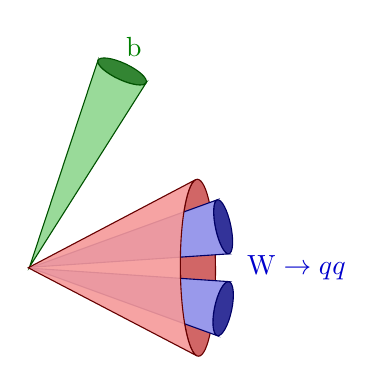
\begin{tikzpicture}
   \def\R{2.5}
  \edef\ang{28}
  \edef\e{0.05}
  \coordinate (O) at (0,0);
  \coordinate (BJ) at ( 65:1.1*\R); % b jet 1
  \coordinate (J1) at ( 12:1.0*\R); % q jet 1
  \coordinate (J2) at (-12:1.0*\R); % q jet 2
  \coordinate (M) at (0:0.85*\R); % merged
  \edef\vang{\pgfmathresult} % angle of vector OV
  \tikzmath{
    coordinate \C;
    \C = (O)-(M);
    \x = veclen(\Cx,\Cy)*\e*sin(\ang)^2; % x coordinate P
    \y = tan(\ang)*(veclen(\Cx,\Cy)-\x); % y coordinate P
    \a = veclen(\Cx,\Cy)*sqrt(\e)*sin(\ang); % vertical radius
    \b = veclen(\Cx,\Cy)*tan(\ang)*sqrt(1-\e*sin(\ang)^2); % horizontal radius
    \angb = acos(sqrt(\e)*sin(\ang)); % angle of P in ellipse
  }
  \coordinate (ML) at ($(M)+(\vang-180:\x pt)+(\vang+90:\y pt)$); % tangency

  % JETS
  \draw[thin,red!40!black,fill=red!70!black!60,rotate=\vang] % base
    (M) ellipse({\a pt} and {\b pt});
  \jetcone[green!80!black]{O}{BJ}{14}{0.10}
  \jetcone{O}{J1}{16}{0.08}
  \jetcone{O}{J2}{16}{0.10}
  \draw[thin,red!40!black,fill=red!90!black!40,fill opacity=0.9,rotate=\vang]
    (ML) arc(180-\angb:180+\angb:{\a pt} and {\b pt})
    -- ($(O)-(\vang:0.03)$) -- cycle;

  \node[green!50!black] at (65:1.24*\R) {b};
  \node[blue!80!black,right] at (0:1.05*\R) {$\mathrm{W} \to qq$};
\end{tikzpicture}
  };
  \node at (4,4)
  {
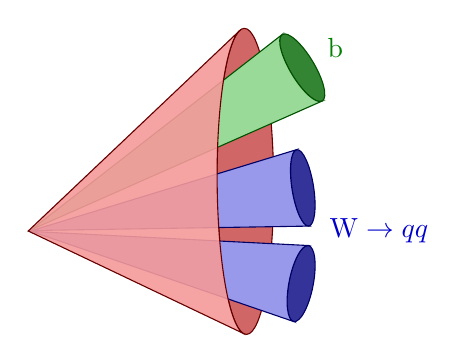
\begin{tikzpicture}
  \def\R{3.5}
  \edef\ang{35}
  \edef\e{0.05}
  \coordinate (O) at (0,0);
  \coordinate (BJ) at ( 31:1.15*\R); % b jet 1
  \coordinate (J1) at (  9:1.00*\R); % q jet 1
  \coordinate (J2) at (-11:1.00*\R); % q jet 2
  \coordinate (M) at (13:0.80*\R); % merged
  \edef\vang{\pgfmathresult} % angle of vector OV
  \tikzmath{
    coordinate \C;
    \C = (O)-(M);
    \x = veclen(\Cx,\Cy)*\e*sin(\ang)^2; % x coordinate P
    \y = tan(\ang)*(veclen(\Cx,\Cy)-\x); % y coordinate P
    \a = veclen(\Cx,\Cy)*sqrt(\e)*sin(\ang); % vertical radius
    \b = veclen(\Cx,\Cy)*tan(\ang)*sqrt(1-\e*sin(\ang)^2); % horizontal radius
    \angb = acos(sqrt(\e)*sin(\ang)); % angle of P in ellipse
  }
  \coordinate (ML) at ($(M)+(\vang-180:\x pt)+(\vang+90:\y pt)$); % tangency

  % JETS
  \draw[thin,red!40!black,fill=red!70!black!60,rotate=\vang] % base
    (M) ellipse({\a pt} and {\b pt});
  \jetcone[green!80!black]{O}{BJ}{14}{0.10}
  \jetcone{O}{J1}{16}{0.08}
  \jetcone{O}{J2}{16}{0.10}
  \draw[thin,red!40!black,fill=red!90!black!40,fill opacity=0.9,rotate=\vang]
    (ML) arc(180-\angb:180+\angb:{\a pt} and {\b pt})
    -- ($(O)-(\vang:0.03)$) -- cycle;

  \node[green!50!black] at (31:1.29*\R) {b};
  \node[blue!80!black,right] at (0:1.05*\R) {$\mathrm{W} \to qq$};
\end{tikzpicture}
  };
  
  \node at (3,-1)
  {
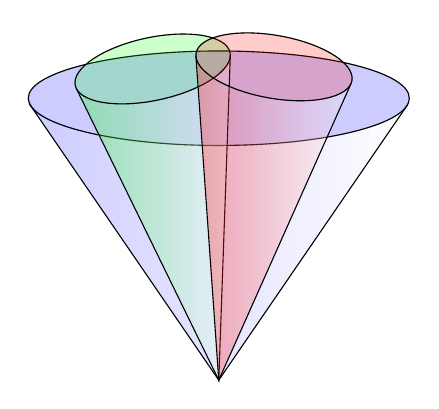
\begin{tikzpicture}

  % AK8 variables
  \def\x{2.4}
  \def\y{3.5}
  \def\R{\x+0.02}
  \def\yc{\y+0.08}
  \def\e{0.6}

  % AK8 cone
  \shade[right color=white,left color=blue,opacity=0.2]
    (-\x,\y) -- (-\x,\yc) arc (180:360:{\R} and \e) -- (\x,\y) -- (0,0) -- cycle;
  \draw[fill=blue,opacity=0.2]
    (0,\yc) circle ({\R} and \e);
  \draw
    (-\x,\y) -- (0,0) -- (\x,\y);
  \draw
    (0,\yc) circle ({\R} and \e);

  % AK4 variables
  \def\x{1.0}
  \def\y{4.0}
  \def\R{\x+0.005}
  \def\yc{\y+0.04}
  \def\e{0.4}

  % AK4 cone 1
  \begin{scope}[rotate=12]
    \shade[right color=white,left color=green,opacity=0.3]
      (-\x,\yc) -- (-\x,\yc) arc (180:360:{\R} and \e) -- (\x,\yc) -- (0,0) -- cycle;
    \draw[fill=green,opacity=0.2]
      (0,\yc) circle ({\R} and \e);
    \draw
      (-\x,\y) -- (0,0) -- (\x,\y);
    \draw
      (0,\yc) circle ({\R} and \e);
  \end{scope}

  % AK4 cone 2
  \begin{scope}[rotate=-10]
    \shade[right color=white,left color=red,opacity=0.3]
      (-\x,\yc) -- (-\x,\yc) arc (180:360:{\R} and \e) -- (\x,\yc) -- (0,0) -- cycle;
    \draw[fill=red,opacity=0.2]
      (0,\yc) circle ({\R} and \e);
    \draw
      (-\x,\y) -- (0,0) -- (\x,\y);
    \draw
      (0,\yc) circle ({\R} and \e);
  \end{scope}

\end{tikzpicture}
  };
  
  \node at (-3,-1)
  {
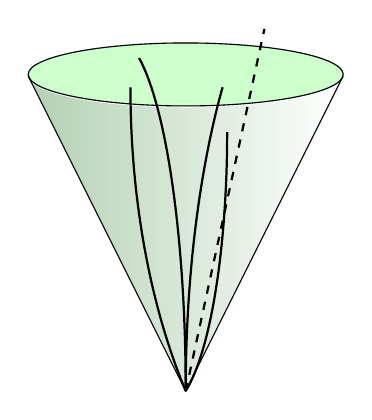
\begin{tikzpicture}

  % cone variables
  \def\x{2.0}
  \def\y{4.0}
  \def\R{\x}
  \def\yc{\y+0.02}
  \def\e{0.4}

  % cone shades + frame
  \shade[right color=white,left color=mygreen,opacity=0.3]
    (-\x,\yc) -- (-2,4) arc (180:360:{\R} and \e) -- (\x,\yc) -- (0,0) -- cycle;
  \draw[fill=green,opacity=0.2]
    (0,\yc) circle ({\R} and \e);
  \draw
    (-\x,\y) -- (0,0) -- (\x,\y);
  \draw
    (0,\yc) circle ({\R} and \e);

  % tracks
  \draw[thick]
    (0,0) arc (320:360:-3 and 6.0); %node[above] {1};
  \draw[thick]
    (0,0) arc (-70:  0:0.8 and 3.5); %node[above] {2};
  \draw[thick]
    (0,0) arc (  0: 70:0.9 and 4.5); %node[above] {3};
  \draw[thick]
    (0,0) arc (180:140:2 and 6.0); %node[above] {4};
  \draw[thick,dashed]
    (0,0) -- (1,4.6);

\end{tikzpicture}
  };
\end{tikzpicture}



\end{document} 